\documentclass{article}
\usepackage[utf8]{inputenc}
\usepackage[russian]{babel}
\usepackage{graphicx}
\usepackage{caption}
\usepackage{float}
\usepackage{hyperref}
\usepackage{xcolor}
\usepackage[unicode, pdftex]{hyperref}
\usepackage[left=2cm,right=2cm,
    top=2cm,bottom=2cm,bindingoffset=0cm]{geometry}
    
\graphicspath{{pictures/}}
\DeclareGraphicsExtensions{.pdf,.png,.jpg}
\definecolor{urlcolor}{HTML}{003bed}
\hypersetup{pdfstartview=FitH, linkcolor=linkcolor,urlcolor=urlcolor, colorlinks=true}

\begin{document}
    % ТИТУЛЬНИК
    \begin{center}
        \hfill \break
        \LARGE{Дискретная математика}\\
        \hfill \break
        \Large{Типовик 4}\\
        \hfill \break
        \hfill \break
        \hfill \break
        \hfill \break
    \end{center}

    \begin{flushright} Ученик: Титов Даниил, M3104 \end{flushright}
    \begin{flushright} Преподаватель: Lipenx \end{flushright}
    \vfill
    \bigskip
    \begin{center} Санкт-Петербург \end{center}
    \begin{center} 2021 \end{center}
    \thispagestyle{empty}
    \newpage
    % СОДЕРЖАНИЕ
    \tableofcontents{}
    \vfill
    \bigskip
    \begin{flushright}
        \href{https://ru.overleaf.com/read/cxvppkhfjptr}{Код на Overleaf}
    \end{flushright}
    \newpage
    % РЕШЕНИЯ
    \section{В кондитерском магазине продавались 4 сорта пирожных: наполеоны, эклеры, песочные и слоёные. Сколькими способами можно купить 7 пирожных?}
        Так как мы знаем:\\
        1. Что нам не важно, в каком порядке мы будем покупать пирожные\\
        2. Что пирожные могут повторяться\\
        То мы будем использовать "Combinations with repetitions":\\
        $ \overline{C^k_n} = \frac{(n+k-1)!}{k!∗(n-1)!} $\\
        $ \overline{C^4_7} = \frac{(7+4-1)!}{4!∗(7-1)!} = \frac{10!}{4!*6!} = \frac{5040}{24} = 210 $
    \section{Сколькими способами можно распределить 150 студентов по 25 человек в группе?}
        Так как мы знаем:\\
        1. Что порядок элементов (студентов) не важен\\
        2. Что студенты не могут повторяться\\
        То мы будем использовать "Combinations"\space 6 раз ($ \frac{125}{25} = 6 $):\\
        $ C^k_n = \frac{n!}{k!∗(n-k)!} $\\
        $ C^{25}_{150} * C^{25}_{125} * C^{25}_{100} * C^{25}_{75} * C^{25}_{50} * 1 = \frac{150!}{25!*(150-25)!} * \frac{125!}{25!*(125-25)!} * \frac{100!}{25!*(100-25)!} * \frac{75!}{25!*(75-25)!} * \frac{50!}{25!*(50-25)!} = \frac{150!}{25!*125!} * \frac{125!}{25!*100!} * \frac{100!}{25!*75!} * \frac{75!}{25!*50!} * \frac{50!}{25!*25!} $
    \section{Сколько различных слов можно получить, переставляя буквы в слове МАТЕМАТИКА?}
        Так как мы знаем:\\
        1. Что нам важно, в каком порядке у нас будут стоять буквы\\
        2. Что мы выбираем все элементы (буквы) в слове\\
        3. Что повторений элементов не может быть\\
        То мы будем использовать "Permutations":\\
        $ P_n = n! $\\
        $ P_{10} = 10! = 3628800 $
    \section{У игрока есть 5 четырёхгранных костей.Сколькими способами может выкинуть ровно две 1 и одну 3 на них, если кости нумерованы?}
        Так как мы знаем:\\
        1. Что нам важно, в каком порядке у нас будут выкинуты кости\\
        2. Что мы выбираем все элементы (цифры) в последовательности\\
        3. Что элементы могут повторяться\\
        То мы будем использовать "Permutations with repetitions":\\
        $ \overline{P_n} (k_1, ..., k_l) = \frac{n!}{k_1!*...*k_l!} $\\
        $ \overline{P_5} (1,1,3,2,2) + \overline{P_5} (1,1,3,2,4) + \overline{P_5} (1,1,3,4,4) = \frac{5!}{2!*1!*1!} + \frac{5!}{2!*1!*2!} + \frac{5!}{2!*1!*2!} = 60 + 30 * 2 = 120 $
        \newpage
    \section{Для представленного графа определите}
        Представленный граф:
        \begin{figure}[h!]
            \fbox{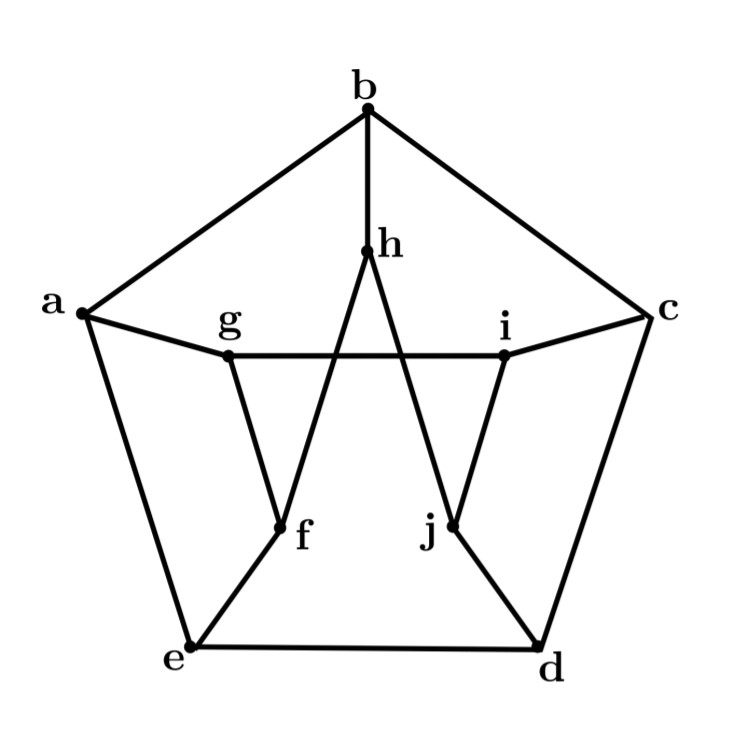
\includegraphics[scale=0.3]{5.jpg}}
        \end{figure}\\
        \subsection{Есть ли в графе Эйлеров цикл или Эйлерова цепь? Если есть, то выпишите. Если нет, то обоснуйте отсутствие}
            \textit{Эйлеров путь в графе} - это путь, проходящий по всем рёбрам графа ровно по одному разу\\
            \textit{Эйлеров цикл} - эйлеров путь, являющийся циклом, то есть замкнутый путь, проходящий через каждое ребро графа ровно по одному разу\\
            Соответственно у нас нет ни Эйлерова пути, ни Эйлерова цикла, так как каждая из вершин имеет нечётную степень
        \subsection{Есть ли в графе Гамильтонов цикл, Гамильтонова цепь? Если есть, то выпишите. Если нет, то обоснуйте отсутствие}
            \textit{Гамильтонов путь} - простой путь (путь без петель), проходящий через каждую вершину графа ровно один раз
            \begin{figure}[h!]
                \fbox{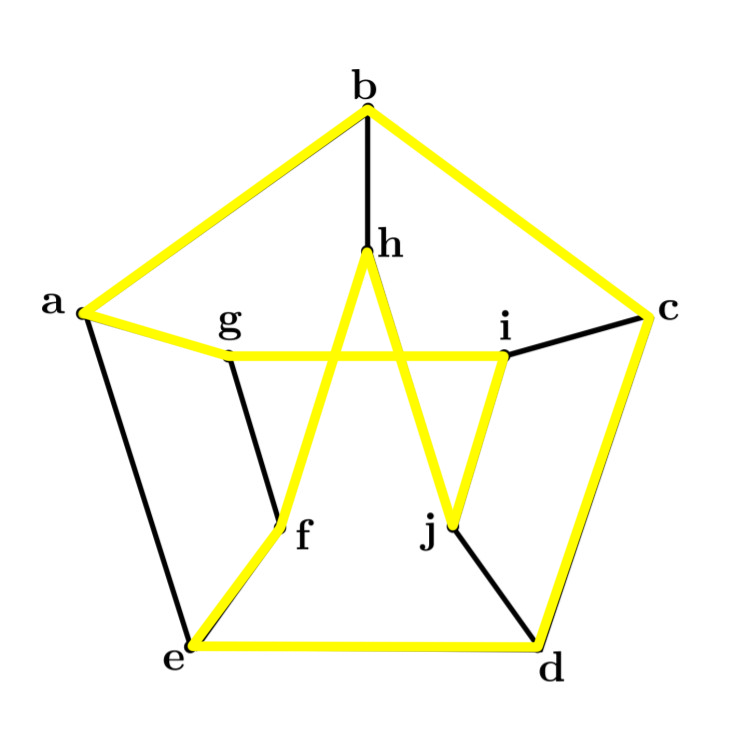
\includegraphics[scale=0.3]{gamCycle.jpg}}
            \end{figure}
            \newpage
            \textit{Гамильтонова цепь} - простой цепь (нет повторяющихся вершин), обладающая свойством гамильтонова пути
            \begin{figure}[h!]
                \fbox{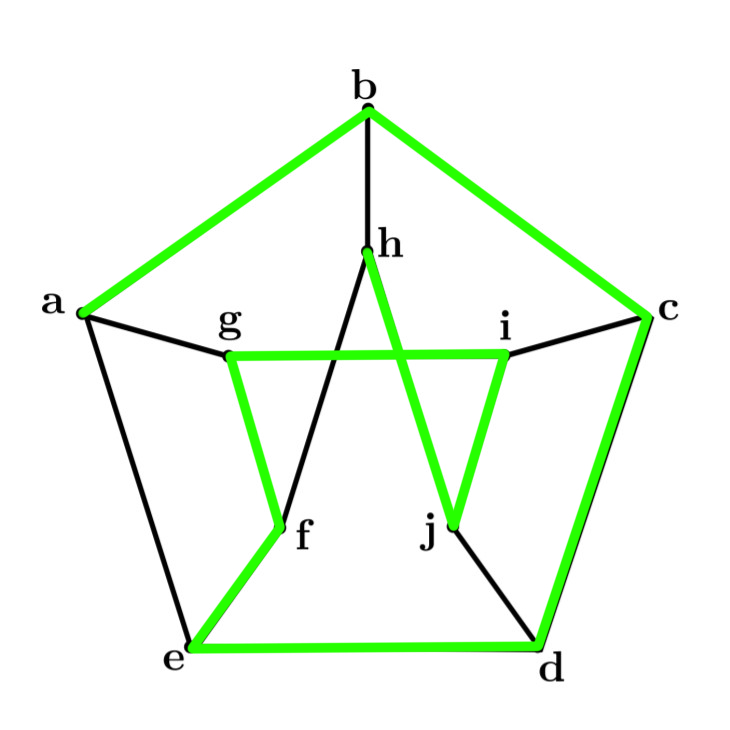
\includegraphics[scale=0.3]{gamChain.jpg}}
            \end{figure}\\
    \section{Нарисуйте орфорграф с 3мя компонентами сильной связности, имеющий не более 11 вершин и не менее 8.}
        Вот мой граф, и тут разными цветами отмечены разные компоненты сильной связности:
        \begin{figure}[h!]
            \center{\fbox{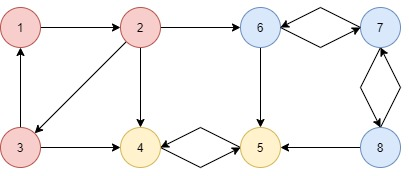
\includegraphics[scale=0.5]{6.jpg}}}
        \end{figure}
    \section{Граф задан матрицей расстояний}
        Матрица:
        \begin{figure}[h!]
            \fbox{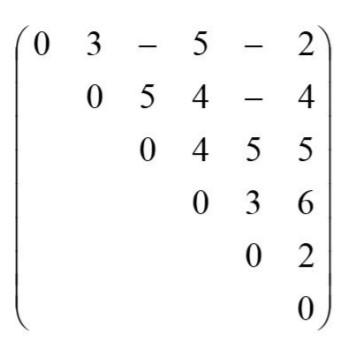
\includegraphics[scale=0.5]{matrix.jpg}}
        \end{figure}
        \newpage
        Граф:
        \begin{figure}[h!]
            \fbox{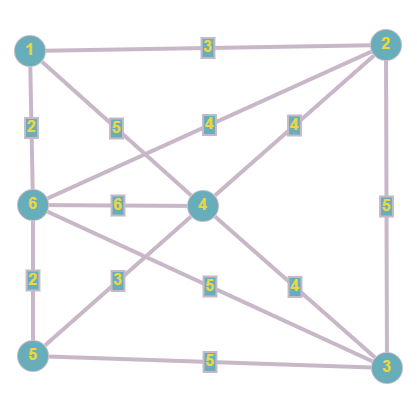
\includegraphics[scale=0.4]{7graph.png}}
        \end{figure}
        \subsection{Построить минимальное остовное дерево}
            \begin{figure}[h!]
                \fbox{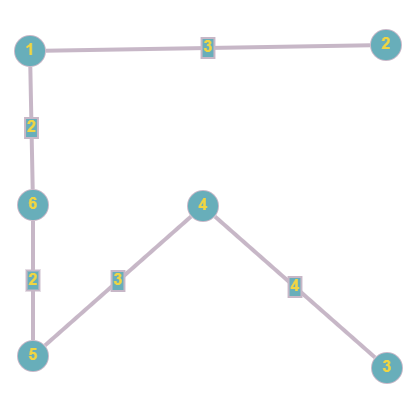
\includegraphics[scale=0.4]{7minSpanTree.png}}
            \end{figure}
        \subsection{Построить фундаментальную систему циклов, ассоциированную с этим остовом}
            \begin{figure}[h!]
                \fbox{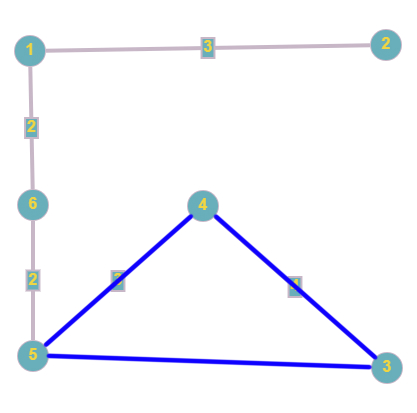
\includegraphics[scale=0.3]{71.jpg}}
                \fbox{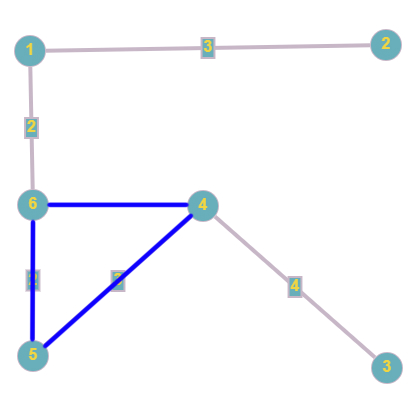
\includegraphics[scale=0.3]{72.jpg}}
                \fbox{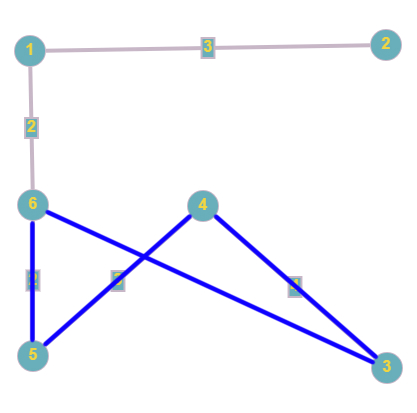
\includegraphics[scale=0.3]{73.jpg}}
                \fbox{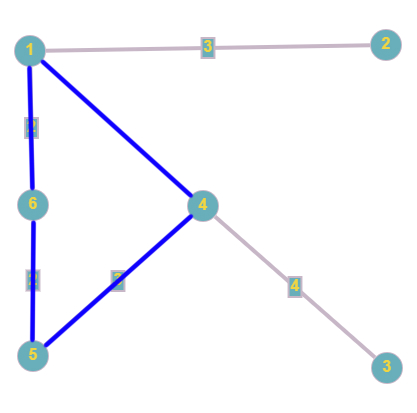
\includegraphics[scale=0.3]{74.jpg}}
                \fbox{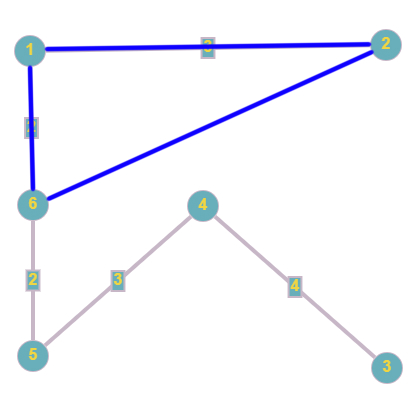
\includegraphics[scale=0.3]{75.jpg}}
                \space\space\space\space\space\space\space\space\space
                \fbox{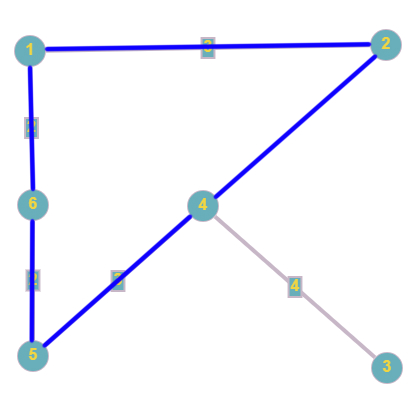
\includegraphics[scale=0.3]{76.jpg}}
                \space\space\space\space\space\space\space\space\space
                \fbox{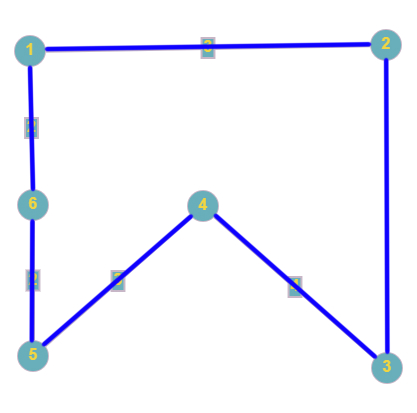
\includegraphics[scale=0.3]{77.jpg}}
            \end{figure}
            \newpage
        \subsection{Найти кратчайшие пути от вершины 4 до всех остальных вершин графа}
            Найти кратчайшее расстояние можно при помощи \href{https://ru.wikipedia.org/wiki/%D0%90%D0%BB%D0%B3%D0%BE%D1%80%D0%B8%D1%82%D0%BC_%D0%94%D0%B5%D0%B9%D0%BA%D1%81%D1%82%D1%80%D1%8B}{алгоритма Дейкстры}, соответственно, используя этот алгоритм, я и получил следующие результаты:
            \begin{figure}[h!]
                \begin{center}
                    \begin{minipage}[h]{0.2\linewidth}
                        \fbox{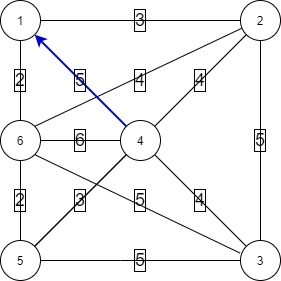
\includegraphics[scale=0.3]{41.jpg}}
                        \caption*{4->1 = 5}
                    \end{minipage}
                    \begin{minipage}[h]{0.2\linewidth}
                        \fbox{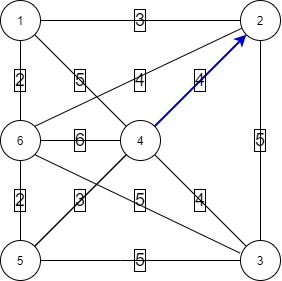
\includegraphics[scale=0.3]{42.jpg}}
                        \caption*{4->2 = 4}
                    \end{minipage}
                    \begin{minipage}[h]{0.2\linewidth}
                        \fbox{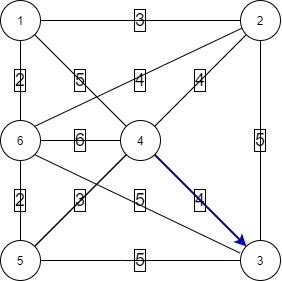
\includegraphics[scale=0.3]{43.jpg}}
                        \caption*{4->3 = 4}
                    \end{minipage}
                    \begin{minipage}[h]{0.2\linewidth}
                        \fbox{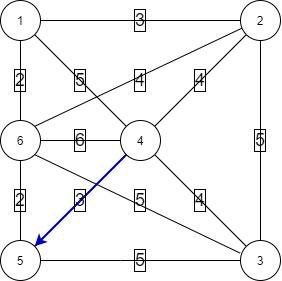
\includegraphics[scale=0.3]{45.jpg}}
                        \caption*{4->5 = 3}
                    \end{minipage}
                    \begin{minipage}[h]{0.2\linewidth}
                        \fbox{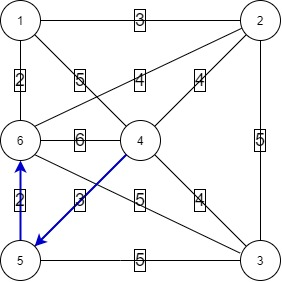
\includegraphics[scale=0.3]{46.jpg}}
                        \caption*{4->6 = 5}
                    \end{minipage}
                \end{center}
            \end{figure}
\end{document}
